\chapter{GIT HISTORY}
To ensure proper version management and collaborative development, the entire project is maintained using Git and hosted on GitHub. This allows for efficient tracking of updates, feature additions, bug fixes, and code reviews. By using Git, different versions of the application can be accessed, making it easy to roll back changes if needed. The repository serves as a centralized location for storing and sharing all project files.

\section{GitHub Repository}

\begin{figure}[H]
    \centering
    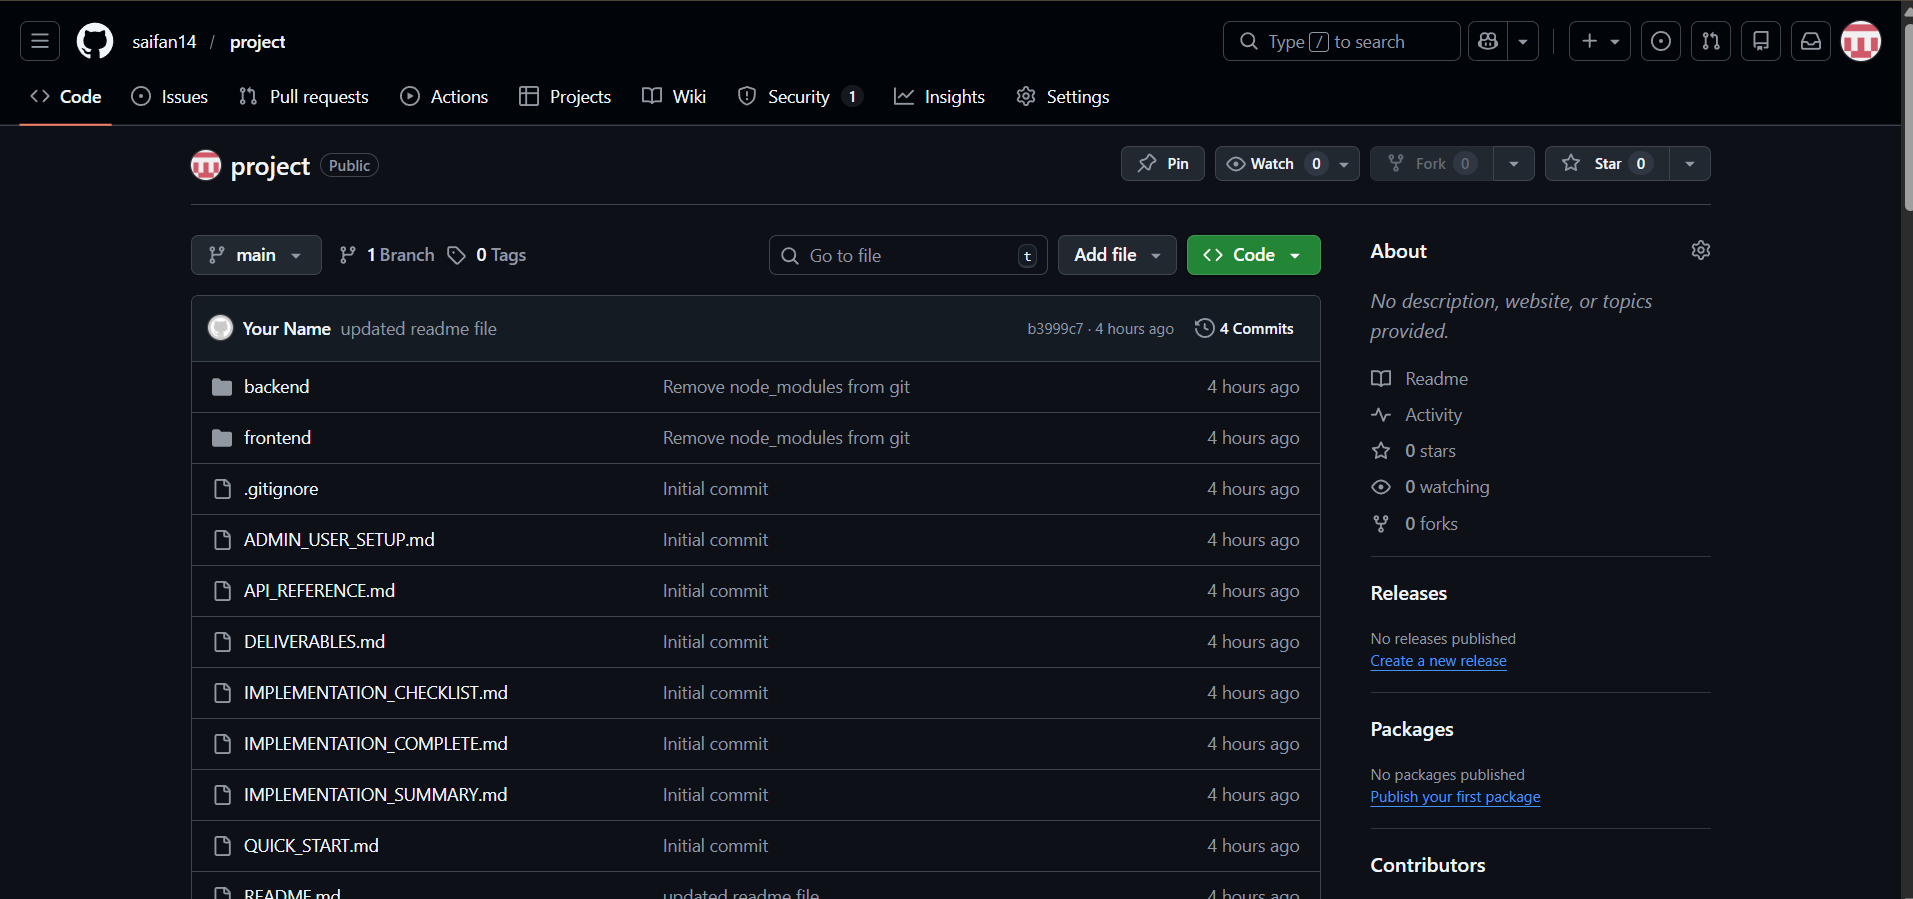
\includegraphics[width=0.95\textwidth]{image/git_repo.png}
    \caption{GitHub Repository Overview}
    \label{fig:git_repo}
\end{figure}

The above screenshot shows the main GitHub repository page with all project files, branches, and recent commit history.

\section{Commit History}

\begin{figure}[H]
    \centering
    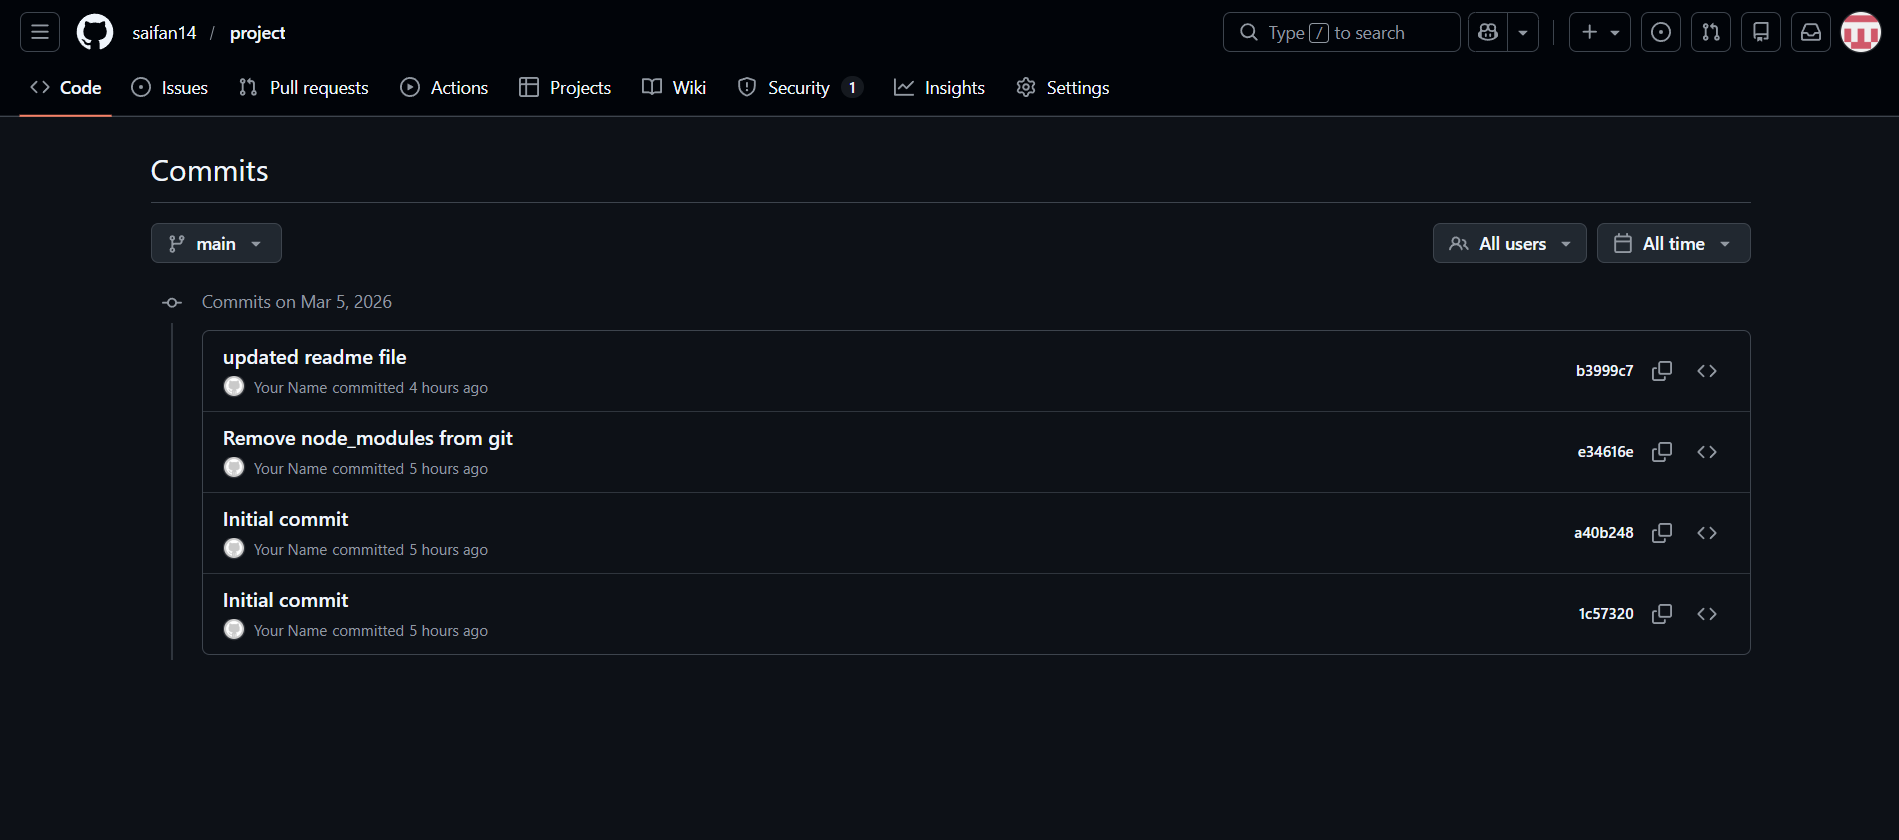
\includegraphics[width=0.95\textwidth]{image/git_commit.png}
    \caption{Git Commit History}
    \label{fig:git_commits}
\end{figure}

The commit history demonstrates the incremental development process, with commits covering feature implementation, bug fixes, documentation updates, and code refactoring across the entire development lifecycle.